\section{Potential participants}
\label{sec:part}

\begin{wrapfigure}{!h}{3.2in}
  \vspace{-0.5cm}
  \centering 
  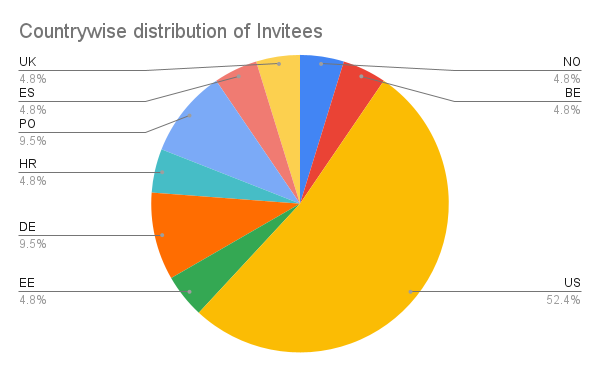
\includegraphics[scale=0.4]{fig/country.png}
  \caption{Country-wise break up of possible participant pool for \sympe.}
  \label{fig:country}
\end{wrapfigure}

We have shortlisted the following individuals as potential
participants in \sympe. We expect to prune this list down markedly to
the numbers we believe ($\sim 30$) which will make the symposium
viable to achieve the goals we have set out for it. It shows a broad
dispersion of disciplines, relevant to ocean observation, gender and
geography. Given the constraints of the symposium, including it being
held while there is substantial uncertainty in how the pandemic
situation will evolve, we believe it would be in the best interests to
narrow the participation to residents of the Americas and Europe. This
is reflected in the detail in Table \ref{tab:part} and is a starting
point to pull together the actual participants.


\begin{table}[H]
  \footnotesize{
\begin{tabular}{|p{3cm}|p{0.5cm}|p{3.5cm}|p{0.5cm}|p{6cm}|}
% {lllll}
  \rowcolor{Gray}
  \bfseries Namem& \bfseries M/F&\bfseries Institution & \bfseries Nationality& Specialization\\
Jo Eidsvik               & M   & NTNU                                  & NO       & Statistical Sampling                            \\
\hline
Aida Alvera Az\'{a}rate    & F   & Univ. of Leige                        & BE       & Remote Sensing, modeling                        \\
\hline
Kanna Rajan              & M   & SIFT LLC \& Univ. of Porto            & PO       & AI, Autonomous systems, Ocean Science           \\
 \hline
Maarja Krusma            & F   & Tallinn Inst. of Tech                 & EE  & Sensors/robotics                                \\
  \hline
Paulo Relvas             & M   & Univ. of Algarve                      & PO       & Physical Oceanography                           \\
\hline
Ralf Bachmeyer           & M   & Univ. of Bremen                       & DE       & Marine robotics, deep sea                       \\
\hline
Yogi Girdhar             & M   & WHOI                                  & US       & Marine robotics + ML                            \\
\hline
Nikola Miskovic          & M   & Univ. of Zagreb                       & HR  & Marine robotics                                 \\
\hline
Maria Joao Ramos         & F   & Univ. of Porto                        & PO       & Bio-Chemistry                                   \\
\hline
Pierre Lermusiaux        & M   & MIT                                   & US       & Modeling                                        \\
\hline
Joao Sousa               & M   & Univ. of Porto                        & PO       & Control Systems + Robotics                      \\
\hline
Ajit Subramaniam         & M   & Columbia Univ.                        & US       & Bio-optics, Oceanography                        \\
\hline
Pere Ridao               & M   & Univ. of Girona                       & ES       & Grasping and control                            \\
\hline
Oliver Zelinsky          & M   & Univ. of Oldernburg                   & DE       & Instrumentation, sensors                        \\
\hline
Peter Girguis            & M   & Harvard                               & US       & Genomics, micro-biology                         \\
\hline
Shubha Satyendernath     & F   & Plymouth Marine Labs                  & UK       & Remote Sensing, Ocean Color                     \\
\hline
Maha Haji                & F   & Cornell                               & US       & Design optimization, Sys. Eng                   \\
\hline
Victoria Orphan          & F   & CalTech                               & US       & Microbial Ecology                               \\
\hline
Kristina Gjerde          & F   & IUCN                                  & US       & Law of the Sea, Env. Law                        \\
\hline
Antonio Pascoal          & M   & Univ. of Lisbon                       & PO       & Control Systems + Robotics                      \\
\hline
Catarina Magahlaes       & F   & CIIMAR, Univ. of Porto                & PO       & Biological Oceanography                         \\
\hline
Rick Stumpf              & M   & NOAA                                  & US       & HABs, Ocean Optics                              \\
\hline
Raphe Kudela             & M   & Univ. of Calif, Santa Cruz            & US       & HABs, remote sensing                            \\
\hline
Katy Croft-Bell          & F   & MIT                                   & US       & Engagement, Exploration                         \\
\hline
Joao Vitorino            & M   & Inst. Hidrografico                    & PO       & Phys. Oceanography, modeling                    \\
\hline
Melissa Omand            & F   & Univ. of Rhode Island                 & US       & Phys. Oceanography                              \\
\hline
Mark Abbot               & M   & Retired/Vermont, former WHOI director & US       & Bio-physical processess, ocean optics           \\
\hline
Renato Mendes            & M   & Univ. of Porto                        & PO       & Physical Oceanography, modeling                 \\
\hline
Chris Roman              & M   & Univ. of Rhode Island                 & US       & Sensors, instrumentation                        \\
\hline
Sarah Webster            & F   & Univ of Washington/APL                & US       & Navigation, Control                             \\
\hline
Julien Brajard           & M   & Sorbonne / Nansen centre              & FR       & data assimilation, machine learning             \\
\hline
Lars Nerger              & M   & Alfred Wegener                        & DE       & Data assimilation                               \\
\hline
Annalisa Bracco          & F   & Georgia Tech                          & US       & Ocean physics, meso-scale dynamics              \\
\hline
Marta Chantal Ribeiro    & F   & UN \& Univ. of Porto                  & PO       & Law of the Sea                                  \\
\hline
Geoff Hollinger          & M   & Oregon State Univ                     & US       & Robotics, Sampling                              \\
\hline
Chelle Gentemann         & F   & Farallon Institute                    & US       & Remote Sensing (SST), air-sea fluxes, saildrone \\
\hline
Ivona Cetinic            & F   & NASA                                  & US       & Remote Sensing (Colour), ocean biogeochemistry  \\
\hline
Matjaz Licer             & M   & NIB                                   & SL & Physical oceanography, ML, modelling            \\
\hline
Pierre-Philippe Mathieux & M   & ESA, Phi-lab (Head)                   & IT       & Remote Sensing, AI                              \\
\hline
Bastien Queste           & M   & U. Gothenburg                         & SE       & Oceanographer, AUVs\\                            
\hline
\end{tabular}
}
  \caption{Potential invitee list (including organizers) to down-select from, for the \sympe.}
  \label{tab:part}
\end{table}

